\section{Protocol overview}
\label{protocol}

Sigma Network organizes protocol state into a blockchain structure. We use a BFT algorithm, described in \autoref{consensus}, to commit a single (possibly empty) block at each height. Because exactly one block is committed at each height, committed blocks form a path. And because all valid blocks at the same height must share the same committed parent, valid blocks form a caterpillar tree.

\begin{figure}[h]
  \centering
    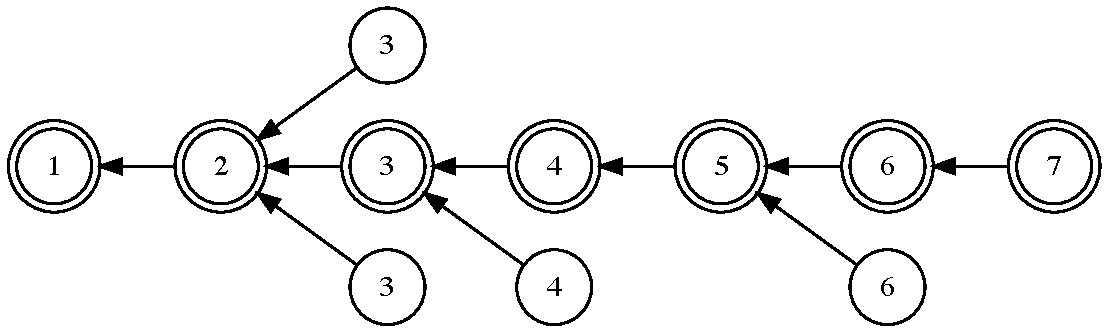
\includegraphics[width=0.7\textwidth]{images/chain-structure}
  \caption{A possible composition of valid blocks. The numbers represent block heights, and the double circles represent committed blocks.}
\end{figure}

This structure has several benefits. Since blocks are committed shortly after they have propagated, transactions are confirmed very quickly, with a strong guarantee of irreversibility. Additionally, blocks can be generated as quickly as the network is able to propagate them; the BFT process eliminates the need for fixed block timing. Finally, the lack of forks makes client performance very predictable.

% TODO: Explicitly define validators.

A validator must register as a block creator before being eligible to create a block, and must register as a voter before being eligible to vote in the BFT consensus protocol. These registration messages are similar to transactions---they must be included in a block before they are recognized, and they may include transaction fees in order to incentivize inclusion.

Each registration message has an associated score, which is pseudorandomly generated based on some account data. An account must have a certain minimum amount of stake, \texttt{DepositAmount}, in order to submit any registrations. The more stake an account has, the more registrations they may submit, each with a unique score.

If more than one validator registers to create the same block, only the one with the highest score is eligible to do so. Similarly, if more than \texttt{MaxVoters} register to vote in the same epoch, only the highest-scoring \texttt{MaxVoters} are eligible to do so.

Blocks are grouped into \emph{epochs}, each consisting of \texttt{EpochSize} blocks. If a validator wishes to participate in epoch $i$, they must submit their registration during epoch $i - 1$. Since there are many blocks in an epoch, validators have many opportunities to have their registration messages included. Censoring registration messages would be difficult, since it only takes a single uncooperating block creator to thwart a censorship attempt by including any pending registrations.
